\documentclass{article}
\usepackage[utf8]{inputenc}

\title{README of CME 211: Homework 4}
\author{Chih-Hsuan Kao, chkao831@stanford.edu}
\date{October 31, 2019}

\usepackage{natbib}
\usepackage{graphicx}

\begin{document}

\maketitle
\section{Class Truss}
Truss class gathers information about a 2D truss at a time, from two files which respectively contain information of joints (number, x/y coordinates, force in x/y direction, a boolean variable indicating whether it has fixed support) and contain information of beams (number and joints on each side). 
Then, using method of joints, the class is capable of plotting a simple 2D plot showing the geometry of the truss as well as calculating beam forces for the truss and print out (to file if an optional command of output filename is given).

\subsection{Methods in Class Truss}
\begin{itemize}
\item init (the constructor)
\begin{itemize}
\item This serves as a constructor in OOP Design. It initializes attributes of class Truss and and takes care of general tasks that are related to the functionality of this class.
\item Type of sparse matrix used: scipy.sparse.coomatrix
\begin{itemize}
\item I chose to use COO matrix such that I could firstly store data as three lists with corresponding elements: row, column, value. 
\end{itemize}
\item Exception Handling: I used numpy.linalg.solve to solve the linear system. Whenever the truss is not a suitable geometry for static equilibrium analysis: 
\begin{itemize}
\item If matrix A is non-square 
\begin{itemize}
\item I would raise RuntimeError("Truss geometry not suitable for static equilibrium analysis") message to command line
\end{itemize}
\item If matrix A is singular
\begin{itemize}
\item I would raise RuntimeError("Cannot solve the linear system, unstable truss?")  message to command line
\end{itemize}
\end{itemize}
\end{itemize}
\begin{itemize}
\item Input parameter(s):
\begin{itemize}
\item inputbeam: file
\begin{itemize}
\item This is a beam file that contains beam information.
\end{itemize}
\end{itemize}
\begin{itemize}
\item inputjoint: file
\begin{itemize}
\item This is a joint file that contains joint information.
\end{itemize}
\item outputfile: string
\begin{itemize}
\item This is a string that specifies the name of output filename.
\end{itemize}
\end{itemize}
\end{itemize}
\begin{itemize}
\item Return(s): None
\end{itemize}
\end{itemize}
\begin{itemize}
\item PlotGeometry
\begin{itemize}
\item This method plots graph showing the geometry of the truss if an optional outputfile name is given in the command line. If given name, a plot would be written to the specified filename.
\item Input parameter(s):
\begin{itemize}
\item outputfile: string
\begin{itemize}
\item This string specifies the outputfile name to which the plot is written. 
\end{itemize}
\end{itemize}
\item Return(s): None
\end{itemize}
\end{itemize}

\begin{center}
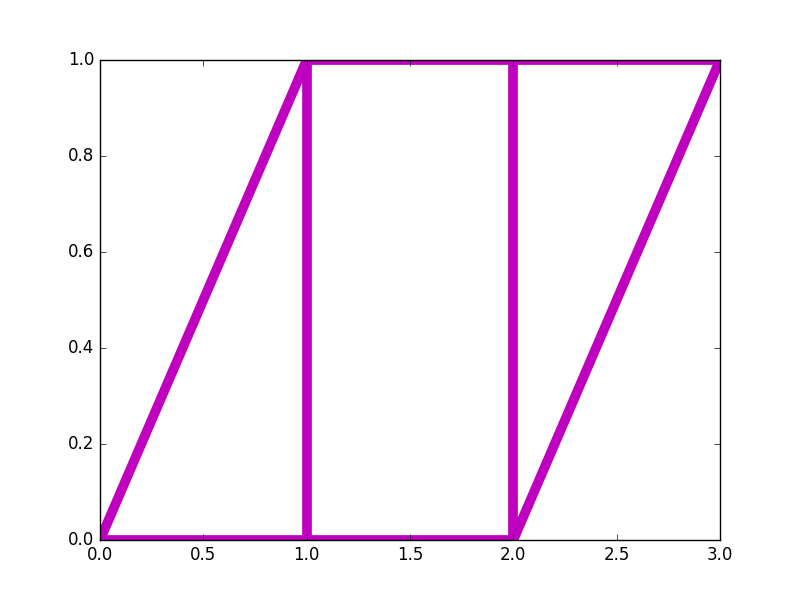
\includegraphics[width=.4\textwidth]{figure1.png}
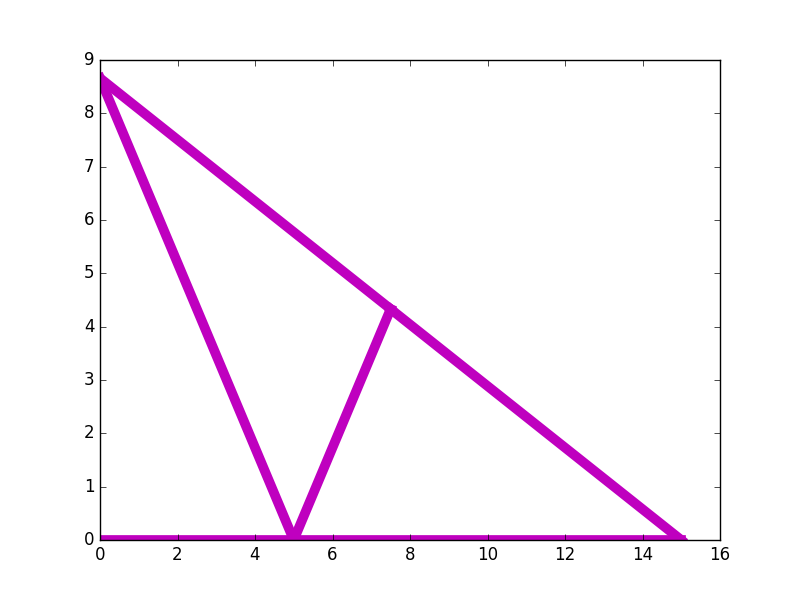
\includegraphics[width=.4\textwidth]{figure2.png}
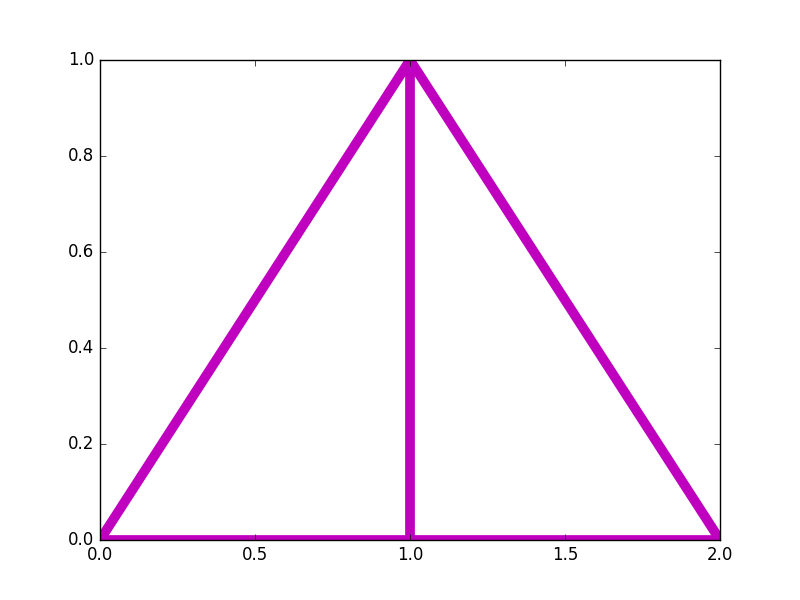
\includegraphics[width=.4\textwidth]{figure3.png}
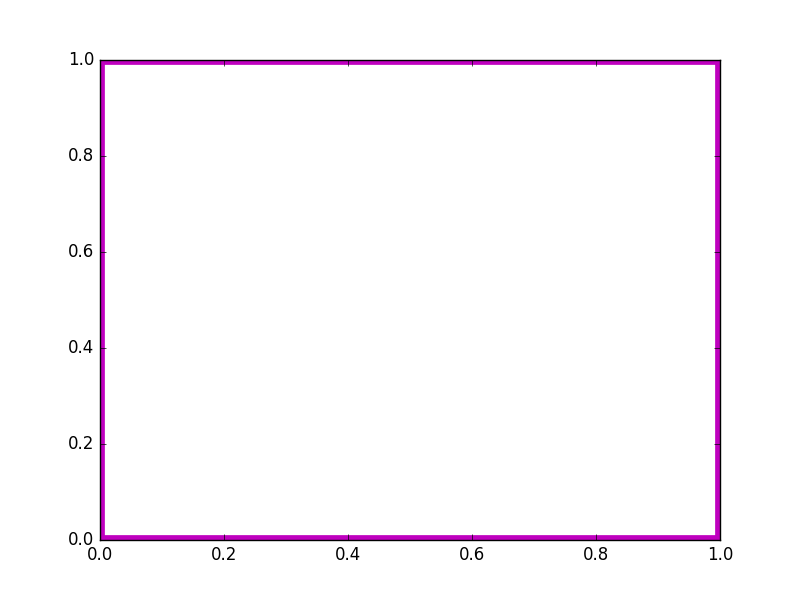
\includegraphics[width=.4\textwidth]{figure4.png}
\end{center}
\caption{  (top left: truss 1; top right: truss 2;}
\caption{bottom left: truss 3; bottom right: truss 4)}

\begin{itemize}
\item CreateJointDict
\begin{itemize}
\item This method returns two dictionaries, in which the number of each joints is key, and its x or y coordinates are values. This method is created for computational usage (part of decomposition).
\item Input parameter(s): None
\item Return(s): 
\begin{itemize}
\item dictx: dictionary
\begin{itemize}
\item This is a dictionary that has joint number as key and its x coordinate as value
\end{itemize}
\end{itemize}
\begin{itemize}
\item dicty: dictionary
\begin{itemize}
\item This is a dictionary that has joint number as key and its y coordinate as value
\end{itemize}
\end{itemize}
\end{itemize}
\end{itemize}
\begin{itemize}
\item CalculateBeamForce
\begin{itemize}
\item This method performs main task of this class. Iterating through each beam, it computes the beam force for 4 entries at each iteration, regarding the value of the entry, the row location, the column location. Those information would be appended to three lists respectively for further usage of COO matrix creation. 
\item Input parameter(s): None
\item Return(s): None
\end{itemize}
\end{itemize}
\begin{itemize}
\item CalculateReactionForce
\begin{itemize}
\item This method handles the last few columns of the matrix. In those columns, reaction force would present if fixed support is there. Firstly, the method would check if a joint has fixed support, if that's the case, the joint number would be saved to a set. Finally, value 1.0 and corresponding location (in matrix) would be appended to lists. 
\item Input parameter(s): None
\item Return(s): None
\end{itemize}
\end{itemize}
\begin{itemize}
\item repr (The string representation method)
\begin{itemize}
\item This overloads the representation method of the class Truss and returns a printable representational string of the given object. When printing out Truss object, the representation string would be printed out to the command line. 
\item Input parameter(s): None
\item Return(s):
\begin{itemize}
\item str: string
\begin{itemize}
\item This string contains the information to be printed to command line when a Truss object is printed.
\end{itemize}
\end{itemize}
\end{itemize}
\end{itemize}
\subsection{OOP Design}
Basically, the attributes within the class Truss are private. This helps encapsulate the data relevant to the Truss class. It gives a strong suggestion not to touch it from outside the Truss class, i.e. any attempt to do so will result in an AttributeError. 

\end{document}
